\documentclass{article}

\usepackage{lipsum}
\usepackage[margin=1.20in,, includefoot]{geometry}
\usepackage{titlesec}
\usepackage{graphicx}

% Specify images directory
\graphicspath{ {./report-images/} }

% Header and Footer stuff
\usepackage{fancyhdr}
\pagestyle{fancy}
\fancyhead{}
\fancyfoot{}
\fancyfoot[R]{ \thepage\ }
\renewcommand{\headrulewidth}{0pt}
\renewcommand{\footrulewidth}{0pt}
\newcommand{\sectionbreak}{\clearpage}
\setlength{\parindent}{0pt}

%

\begin{document}
\begin{titlepage}
	\begin{center}
	\line(1,0){300}\\
	[0.25in]
	\huge{\bfseries Data Fitting Report}  \\
	[2mm]
	\line(1,0){200} \\
	[1.5cm]
	\Large{Exercise 3} \\
	[0.25cm]
	\Large{Comparison between interpolating polynomial and natural cubic spline} \\
	[12cm]
	\end{center}
	\begin{flushright}
	\large{Cesare De Cal \\
	[0.25cm]
	Professor: Annie Cuyt \\
	[0.25cm]
	Assistant Professor: Ferre Knaepkens \\
	}
	\end{flushright}
\end{titlepage}

\section{Introduction}\label{sec:intro}
An imaginary chemistry experiment produces the following data:

  \begin{table}[!ht]
    \large        %% not "\fontsize{12}{12}\selectfont"
    \centering    %% not "\center{...}"
    \begin{tabular}{|c|c|c|c|c|c|c|c|}
    \hline
    \it{x}\textsubscript{i}&-1&-0.96&-0.86&-0.79&0.22&0.50&0.93\\     %% no "&" at start of row
    \it{f}\textsubscript{i}&-1.000&-0.151&0.894&0.986&0.895&0.500&-0.306\\
    \hline        %% extra \hline at bottom of table
    \end{tabular}
  \end{table}

The goal of this exercise is to use these data points to compute and plot the interpolating polynomial together with the natural cubic spline, and to report what it is observed. In the following sections I am going to describe the tools used to compute and plot the interpolating polynomial and the natural cubic spine, and draw conclusions based on the plot.

\section{Tools}
The following programming language and libraries have been used in this exercise:
\begin{itemize}
  \item Python 3.7
  \item SciPy
\end{itemize}
The following NumPy methods of the SciPy environment have been used in this exercise:
\begin{itemize}
  \item numpy.array
  \item numpy.linspace
  \item numpy.polynomial.polynomial
  \end{itemize}
The following Matplotlib methods of the SciPy environment have been used in this exercise:
 \begin{itemize}
  \item matplotlib.pyplot.plot
  \item matplotlib.pyplot.legend
  \item matplotlib.pyplot.show
  \end{itemize}
This report was written in \LaTeX. The results produced by the SciPy library were checked using Maple.
  
\section{Computing the interpolating polynomial}
To compute the interpolating polynomial, I use the Lagrange method which is one of the methods saw in class. I'll also calculate the roundoff errors and the errors on the coefficients. \\
The polynomial found is: \\
[0.25cm]

The coefficients are: 
 \begin{itemize}
  \item 0.04365005085
  \item 16.0766955610565
  \item -0.048402197837630
  \item -20.10047681678335740
  \item 0.0168806991536721320
  \item 5.029463735952404423200
  \item -0.006446071786954468800
  \end{itemize}

Here's a graph showing the 6th degree interpolating polynomial:

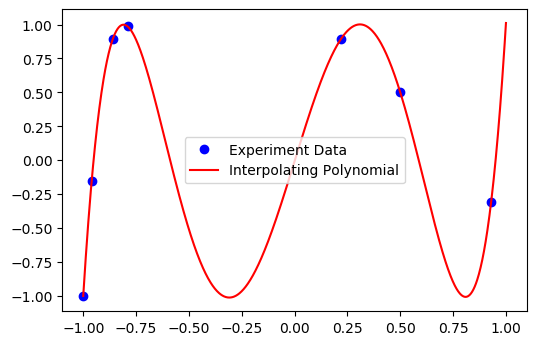
\includegraphics{intpoly}

\end{document}